%//////////////////////////////////
%/// P R E A M B L E

\documentclass[a4paper, 12pt]{article}

\usepackage{geometry}
\usepackage[utf8]{inputenc}
\usepackage[singlespacing]{setspace}
\usepackage{amsmath}
\usepackage{mathtools}
\usepackage{caption}
\usepackage{float}
\usepackage{booktabs}
\usepackage{graphicx}
\usepackage{multicol}
\usepackage{gensymb}
\usepackage{breqn}
\usepackage{indentfirst}
\usepackage{siunitx}
\usepackage{tabularx, booktabs}
\usepackage[calcwidth]{titlesec}
%\newcolumntype{Y}{>{\centering\arraybackslash}X}
\usepackage{xcolor}
\usepackage{pdfpages}

\usepackage{multicol}
%\usepackage{supertabular}

\usepackage{svg}

\widowpenalty = 4500
\clubpenalty  = 4500




\newcommand*\dif{\mathop{}\!\mathrm{d}}
\newcommand*\shortminus{\scalebox{0.5}[1.0]{\( - \)}}
\newcommand{\hspa}{\hspace{0.02128623625220817\paperwidth}}
\newcommand{\hspb}{\hspace{0.013155617496424828\paperwidth}}

\definecolor{hsblue}{HTML}{0cb5df}
\definecolor{hsblueshade}{HTML}{b6e9f5}


%%========================================
%% circuitikz properties
\usepackage[european, straightvoltages]{circuitikz}
%\ctikzvalof{voltage/distance from node = .2}
%\ctikzset{voltage/distance from node  =.5}% in \pgf@circ@Rlen units
%\ctikzset{voltage/distance from line  =.25}% pos. between 0 and 1
%\ctikzset{voltage/bump b/.initial     =1.5}%

\ctikzset{current/distance            = .618}


%%========================================

%%
%% Path settings
%%
\graphicspath{ {./graphics/} }

\geometry{
 a4paper,
 total={0.6180339887498948\paperwidth,0.6180339887498948\paperheight},
 top = 0.1458980337503154\paperheight,
 bottom = 0.1458980337503154\paperheight
 }

\linespread{1.1458980337503154}

\titleformat{\section}[hang]{\Large\bfseries}{\thesection\hspb\textcolor{hsblueshade}{|}\hspa}{0pt}{\Large\bfseries}

\setlength{\parskip}{0.013155617496424828\paperheight} % paragraph spacing

\titlespacing{\section}       {0em}{0em}{0em}
%\titlespacing{\subsection}   {0em}{.50em}{.25em}
%\titlespacing{\subsubsection}{0em}{.50em}{.25em}
%\titlespacing{\paragraph}    {0em}{.25em}{.25em}

%//////////////////////////////////
%/// D O C U M E N T
\begin{document}

%%%%%%%%%%%%%%%%%%%%%%%%%%%%%%%%%%%%%
  %\includepdf{Deckblatt.pdf}
  
\includepdf{./titlepage/titlepage.pdf}
  \clearpage
  \setcounter{page}{1}
%%%%%%%%%%%%%%%%%%%%%%%%%%%%%%%%%%%%%

\section{Vorbereitungsaufgaben}


  \subsection{}

  \begin{center}

    \subsubsection*{Spule}
    \large Reihenmodell

      \begin{circuitikz}

        \draw (-0.3819660112501051,0) to[R, l=$R_{sL}$, o-] (1.6180339887498948,0);
        \draw (1.6180339887498948,0) to[L, l=$L_s$, -o] (1.6180339887498948*2+0.3819660112501051,0);

      \end{circuitikz}
    \end{center}

  \begin{center}
    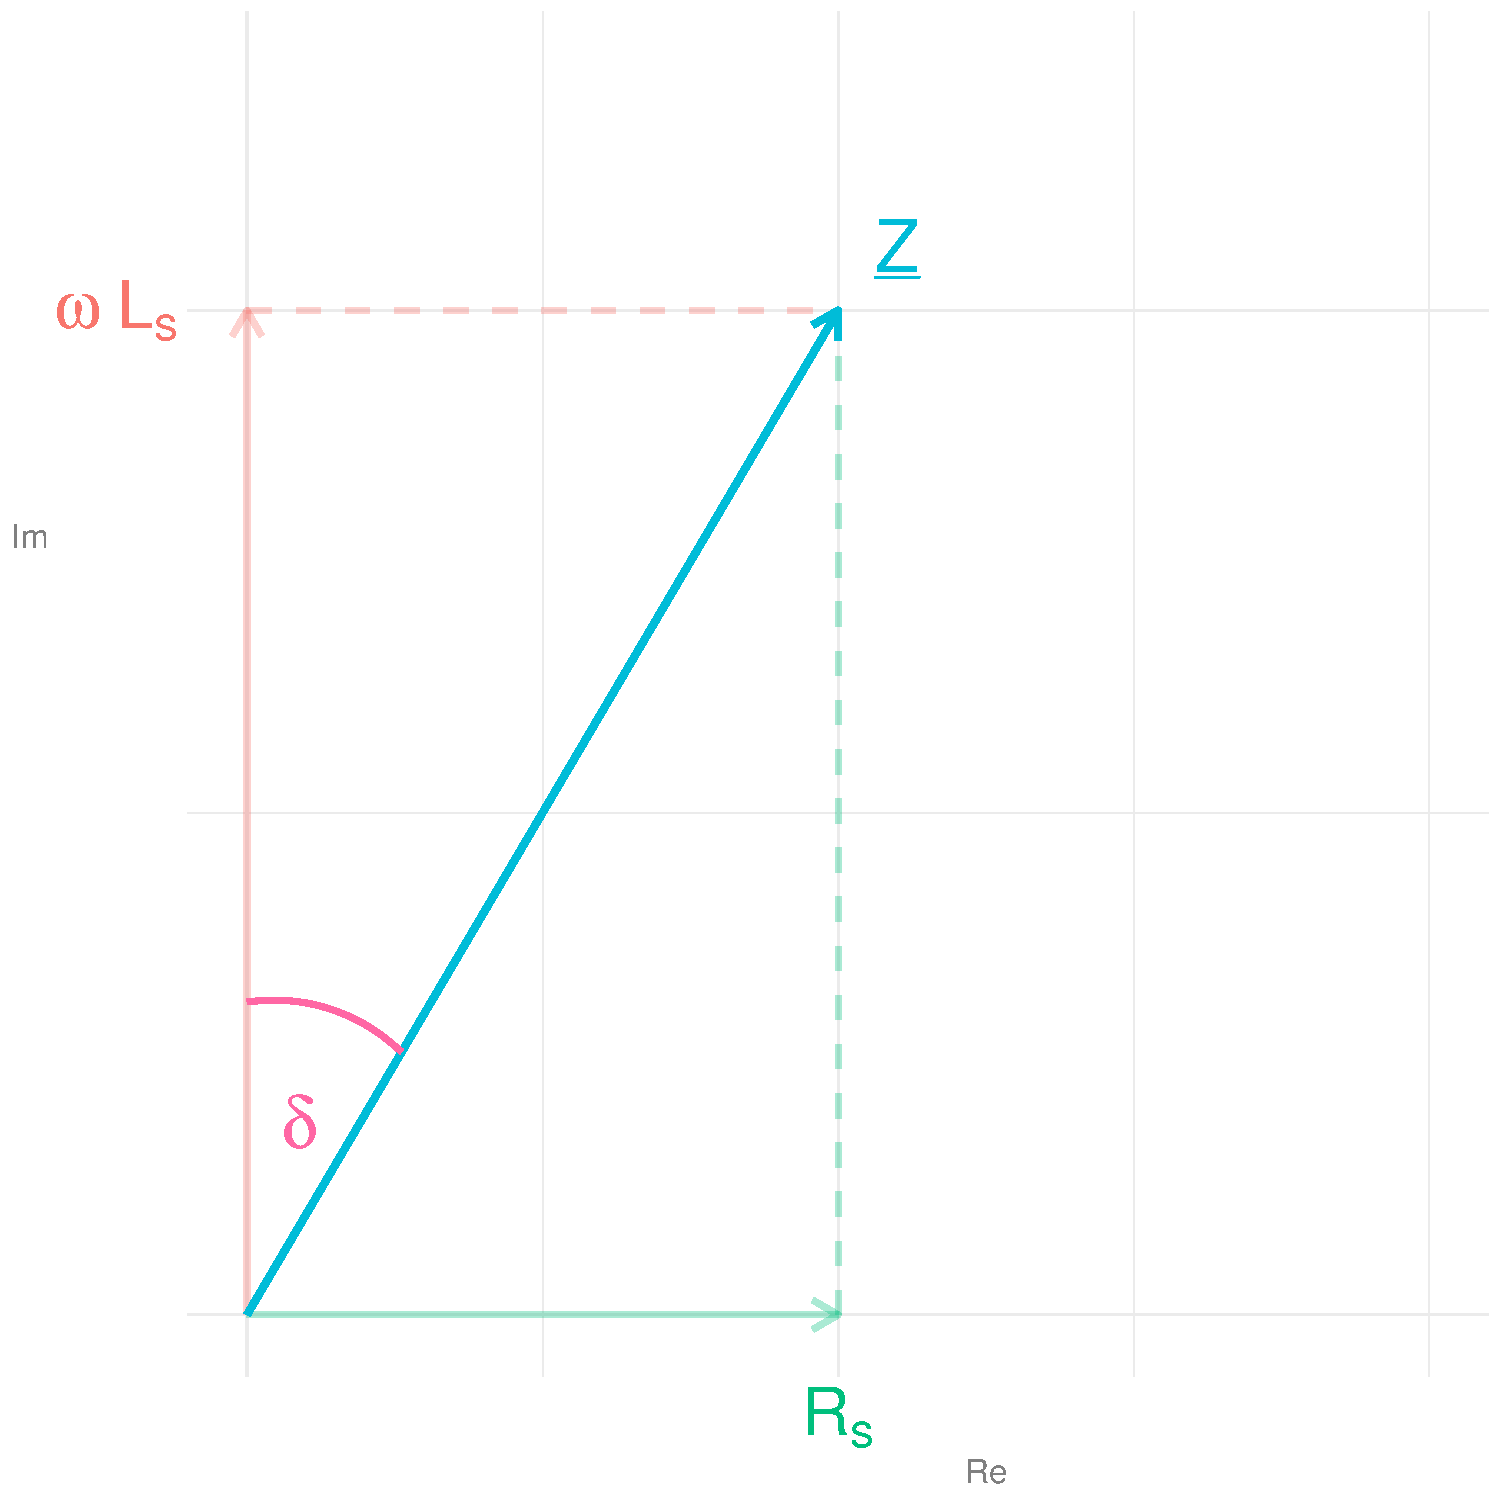
\includegraphics[scale=0.3819660112501051]{./R/2_1/ESBs_Spule.pdf}
  \end{center}

  Der Verlustwinkel $\delta$ ist der Winkel der Spulenimpedanz mit der imaginären Achse der gaußschen Zahlenebene. $\tan{\delta}$ wird auch Verlustfaktor $d$ genannt.

  $$\tan{\delta} = \frac{\omega L_s}{R_{sL}}$$

  Die Güte $Q$ der realen Induktivität ist demnach als der Kehrwert des Verlustfaktors definiert:

  $$ Q_{Ls} = \frac{1}{\tan{\delta}} = \frac{R_{sL}}{\omega L_s}$$

  % Parallelmodell Spule
  \vspace{0.013155617496424828\paperheight}
  \begin{center}
  \large Parallelmodell

    \begin{circuitikz}

      \def\innerwidth{3}
      \def\innerheight{\innerwidth*0.3819660112501051}
      \def\klemmlength{\innerheight*0.6180339887498948}

      \draw (0,\innerheight/2)  to[R, l=$R_{pL}$] (\innerwidth,\innerheight/2);
      \draw (0,-\innerheight/2) to[L, l=$L_p$] (\innerwidth,-\innerheight/2);
      \draw (-\klemmlength,\klemmlength/4) to[short, o-] (0,\klemmlength/4);
      \draw (0,-\innerheight/2)  to[short] (0,\innerheight/2);
      \draw (\innerwidth,-\innerheight/2)  to[short] (\innerwidth,\innerheight/2);
      \draw (\innerwidth,\klemmlength/4) to[short, -o] (\innerwidth+\klemmlength,\klemmlength/4);

    \end{circuitikz}
  \end{center}

  \begin{center}
    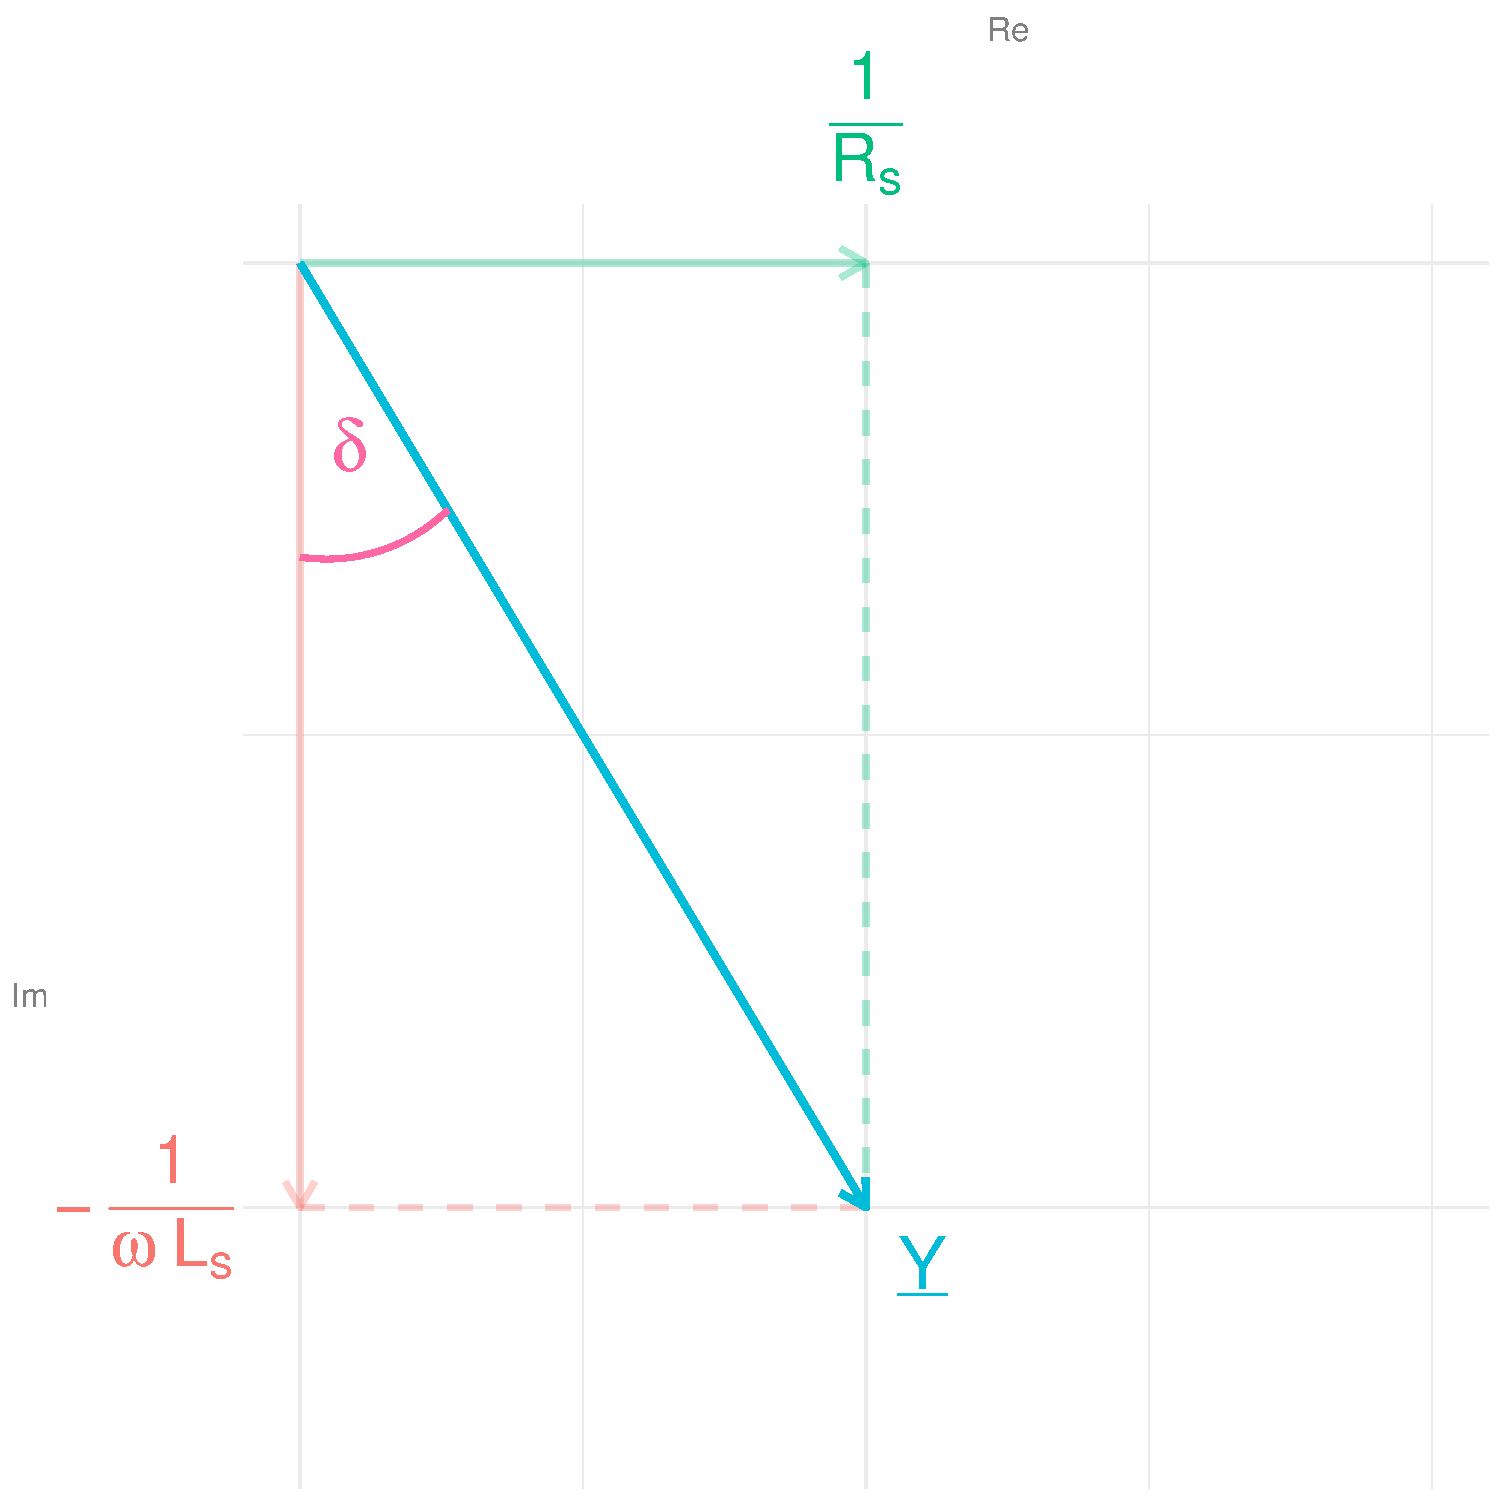
\includegraphics[scale=0.3819660112501051]{./R/2_1/ESBp_Spule.pdf}
  \end{center}


  \subsubsection*{Kondensator}
  % Reihenmodell Kondensator
  \begin{center}

    \large Reihenmodell

      \begin{circuitikz}

        \draw (-0.3819660112501051,0) to[R, l=$R_{sC}$, o-] (1.6180339887498948,0);
        \draw (1.6180339887498948,0) to[C, l=$C_s$, -o] (1.6180339887498948*2+0.3819660112501051,0);

      \end{circuitikz}
    \end{center}

    % Parallelmodell Kondensator
    \vspace{0.013155617496424828\paperheight}
    \begin{center}
    \large Parallelmodell

      \begin{circuitikz}

        \def\innerwidth{3}
        \def\innerheight{\innerwidth*0.3819660112501051}
        \def\klemmlength{\innerheight*0.6180339887498948}

        \draw (0,\innerheight/2)  to[R, l=$R_{pC}$] (\innerwidth,\innerheight/2);
        \draw (0,-\innerheight/2) to[C, l_=$C_p$] (\innerwidth,-\innerheight/2);
        \draw (-\klemmlength,\klemmlength/4) to[short, o-] (0,\klemmlength/4);
        \draw (0,-\innerheight/2)  to[short] (0,\innerheight/2);
        \draw (\innerwidth,-\innerheight/2)  to[short] (\innerwidth,\innerheight/2);
        \draw (\innerwidth,\klemmlength/4) to[short, -o] (\innerwidth+\klemmlength,\klemmlength/4);

      \end{circuitikz}
    \end{center}
\section{Versuchsaufgaben}


\end{document}
